% Formato modificado por CORUM para la escritura de artículo

% Si es formato ieee descomentar la siguiente linea
\documentclass[journal,transmag]{IEEEtran}

\usepackage[utf8]{inputenc}
%\usepackage[spanish]{babel}
\usepackage{amsmath}
\usepackage{amsfonts}
\usepackage{amssymb}
\usepackage{graphicx}
%\usepackage[colorlinks,hyperindex,linkcolor=red,urlcolor=blue]{hyperref}
\usepackage{hyperref}
\usepackage{setspace}
\usepackage{subfig}
\usepackage{url}         

\usepackage{epsfig}

%ruta para guardar las imagenes
\graphicspath{ {figuras/} }

\begin{document}
\title{Educational Platform for Sexuality, for the Project ``Red Sentir... Con-ciencia juvenil''}

\author{\IEEEauthorblockN{J. A. Gómez Múnera\IEEEauthorrefmark{1,2}, and
A. Giraldo\IEEEauthorrefmark{1,2}}
\IEEEauthorblockA{\IEEEauthorrefmark{1}Corporación Estudiantes Universitarios y Profesionales de Marinilla (CORUM) \\Calle 30 San José N$\circ$ 25-118, Marinilla - Antioquia, Colombia}
\IEEEauthorblockA{\IEEEauthorrefmark{2} Grupo de Desarrollo Rural, Instituto Tecnológico COREDI \\ Calle 30 N$\circ$ 36-11, Marinilla - Antioquia, Colombia
\\ \href{mailto:gomezmunera@corum.org.co}{gomezmunera@corum.org.co}, \href{mailto:alejo@corum.org.co}{alejo@corum.org.co}}
\thanks{Manuscript received December 1, 2018; revised August 26, 2015. 
Corresponding author: J. A. Gómez(email: gomezmunera@corum.org.co)}}

% The paper headers
\markboth{Transactions on Education ,~Vol.~14, No.~8, December~2018}%
{Gómez \MakeLowercase{\textit{et al.}}: Bare Demo of IEEEtran.cls for IEEE Transactions on Magnetics Journals}

% make the title area
\maketitle

\begin{abstract}
\textbf{\textit{Abstract}}---Within the national development plan 2014-2018 of Colombia considered education as a fundamental pillar, where the same plan served as a mechanism that would allow social equality and thus levelling the possibilities of all Colombians. Taking this into account, and considering the accelerated increase in the use of information technologies and the communication, along with the possibility of providing more coverage in education, such as ``La Corporación de estudiantes universitarios y profesionales de Marinilla (CORUM)'' development and implemented a project called ``Red Sentir ... Con-ciencia Juvenil'' focused on the prevention of adolescent pregnancy, strengthening of the life plan, critical thinking, autonomy and making conscious decisions. The project derives in three fundamental components that constitute a process of integral formation with young people between 10 and 19 to us from the eastern Antioquia, that allows them to interact and relate with parents, teachers and institutional agents. The components mentioned are: $(i)$ formation and socialization, $(ii)$ regional bureau, and $(iii)$ a digital platform. In this article, emphasis is placed on the strategies and developments made by the digital component in the creation of a virtual environment that allows linking experts, teachers, youth, parents and health institutions. For the development, a social network was created through different technologies, which involve web development, creation of relational database, server configuration and development of video game. All this possible through different languages of programming.
\end{abstract}

\begin{IEEEkeywords}
Education platform, sexual education, teenage pregnancy, family planning health service, young friendly health service, sexual health services and reproductive, sexual education.
\end{IEEEkeywords}

%\IEEEdisplaynontitleabstractindextext
\IEEEpeerreviewmaketitle

\section{INTRODUCTION}

In Colombia, fertility in adolescence became in a public health problem, when from 1990 (for adolescents between 15 and 19 years old) measures of $12.8\%$, presenting in the later years a tendency systematically increasing that finds the maximum value in 2005 $(20.5\%)$. For the year 2010 ($19.5\%$) a trend was achieved-decreasing that continues to be presented in 2015 with a measure of $17.4\%$. It is expected that by the year 2021 according to the adjustment made to the Ten-Year Public Health Plan 2012-2021 we reach the reduction of that percentage to a $15\%$~\cite{Pro2015}. By such a reason, Colombia was raised in the development objectives of the Millennium (ODM) have cups of teen pregnancy by below $15\%$, however, the percentages reached were very far from those figures, which makes it necessary to redouble the efforts to reduce pregnancy in adolescents. In 2013, Colombia registered 6,423 births in women among 10 and 14 years and almost 150 thousand in women between 15 and 19 years, a figure that is high if you consider that together they represent $23.5\%$ of all birth~\cite{PNUD2015}.

Efforts to reduce adolescent pregnancy have been most significant in the most socially advantaged groups, in opposition to the less favoured, causing expand socio-economic gaps. This reflects the need to make greater efforts of the policy of prevention of teenage pregnancy in lesser groups favoured socially and where the greatest prevalence of adolescent pregnancy~\cite{Pro2015, Pro2015II}: rural areas, less educated, situations of poverty.

The differences caused by socioeconomic situations and geographical location, show that actions must be taken or generate inclusion strategies social~\cite{BID2017}, in which the topics of education are addressed sex in a cross-cutting manner with a rights-based approach and with greater coverage, to allow for the reduction of the existing gaps confirmed in the national plan of 2014-2018 development, and the principle of "do not leave anyone behind" enshrined in the 2030 Agenda, which includes the Objectives of Sustainable Development (ODS).

The problem of teenage pregnancy in Colombia shows that only $9\%$ of women and $5\%$ of young men consult health services because of mistrust and ignorance of this system. Despite that teenagers are aware of the methods contraceptives, only a small portion are used, according to figures published in~\cite{Pro2015II}, for the age range between 15-19 years, in women it is around $30\%$ and in $47\%$ men. The use of contraceptive methods not only it is important to control the birth rates of the country but also to prevent transmission infections sexual, in this sense, the use of the condom in Colombia is one of the safest practices to prevent diseases of 'sexual transmission ($85.1\%$ in men and $84.4\%$ in women).
 
When the problem is approached from an approach of rights and to respond to information needs and formation in sexuality issues, it is necessary to raise education in a holistic way, in which they are strengthen and promote empowerment and develop skills in young people from a critical perspective that allows them make decisions that make it possible to protect and guarantee their sexual and reproductive rights. The exercise of sexuality it is a human quality, whose effective construction requires intentional, structured processes or strategies and systematics that facilitates information and formation on issues related to sexuality analysed in the different geographic and socio-economic environments beyond the lived at school.

Responding to the needs described above, was created the "Red Sentir ... Con-Ciencia Juvenil". The project, aims to implement strategies to prevent teen pregnancy focusing in strengthening the life plans of young people,linking digital tools in 6 municipalities from Eastern Antioquia - Sonson, Abejorral, San Francisco,Marinilla, San Luis and Algeria-, this through the development of a virtual educational and recreational platform, what includes components for social networks, mobile devices and video games, where it focuses on sexual education and the strengthening of the projects that make up the plans of life of young people.

The project works with 3 components that are: $(i)$ Digital Platform, $(ii)$ Formation and Socialization and $(iii)$ Regional Bureau.These components allow strategies to be activated pedagogics from technology, memory and research, with which a pedagogical addressing is achieved that produces comprehensive, holistic and meaningful educational processes. The Formation and socialization components and that of Regional bureau are linked to the component digital through the strategy of realization of the digital platform, in said platform is documented and the contents addressed within the courses are reflected made, as well as reviews on the encounters of the different municipalities. 

%On the part of the Regional Bureau it is related through the visualization of each one commitments of the municipalities with the processes of the ``Red Sentir''.

The strategy of the Sentir Network was based on working on the determinants of teenage pregnancy, with which changes can be achieved in the initial situation and reach reductions in teen pregnancy rates in the region from eastern Antioquia. This is because it includes a methodology where the activities that are carried out promote interaction with young people and their environments, which configures a determining factor in favouring a relationship of trust and quality with the young person by a trainer who can act at the motivational level and in turn serve as a reference and/or model. This provides a peaceful environment for young people, where they take ownership of the topics discussed and allow them interact safely to address important aspects in order to encourage assertive behavioural changes. 

%Despite the need to implement ICT by expanding its access and appropriation, it is indisputable that there are abysmal inequalities in terms of the possibility of access to same in Latin America, which make up a gap digital in two dimensions: On the other hand, the international gap existing where there is a Latin American backwardness regarding the progress of ICT in the most developed countries and on the other, the inequalities within the same countries Latin American countries usually related to the level of income, the quality of life and family cycles~\cite{Sunkel2006}, decrease this gap requires a relevant integration of ICT's with education as well as the use, update, and interpenetration of specific sociocultural contexts.
%
%In Colombia, according to what is established in~\cite{Plan2014}, wanted promote the use, understanding, appropriation and interaction of ICTs, thus seeking to generate guarantees for society to access different services, doing in this way that the people of the country can be an active part of society of knowledge. Giving preponderance to the use of ICT and linking this with educational issues, it will be possible to reduce the socio-economic gaps and give young people opportunities for an integral development with quality of life. 

The main features of the platform ``Red Sentir'', that makes it different from other websites or platforms virtual identities (such as those of the protection ministry) and health of the Colombian government~\cite{PagGob2018}, that of the secretary of health of Bogota in alliance with the Foundation Santa Fe de Bogota and Profamilia~\cite{Sexperto2018}, or the Frequent Questions about health~\cite{1DOC3}) are: $(i)$ pleasantly generated content for adolescents and young people, $(ii)$ active participation interaction among youth, $(iii)$ video games for the compression of sexuality, $(iv)$ discretion of the environment to encourage the participation of young people by offering the possibility of participating anonymously, and $(v)$ the deployment of different interfaces according to the interests of each public (young or adult).

\section{OBJECT}\label{sec:propositos}

The ``Red Sentir'' Digital Platform is designed to attract young people through videos, animations and two video games, which can be accessed from the web and mobile devices. The platform also makes it possible for the municipal and departmental health and education secretariats to articulate and use it as a means of disseminating their sexual and reproductive health programmes, offering them the possibility of using the didactic guides for the training of parents and teachers. The platform was designed in the Creative Commons format, which has allowed developers to easily link to the platform.

The ``Red Sentir'' project, linked the users through the exchange of concepts and experiences learned within the courses and allows to continue with the process of learning and empowerment of the themes of sexuality, life plan, dreams and recognition of the body as first territory (Other works such as~\cite{zeck2007impact} impact shows a study about the impact of teenage pregnancy on the future life and the social, family and educational changes). To take this to different modules have been programmed that allow a constant interaction between and you can find a different display depending on the age of the registered user.

In the case that the user be a young person, has the following modules: $(i)$ a Timeline, $(ii)$ young friendly health services, $(iii)$ frequent questions, $(iv)$ forums, and finally $(v)$ two video games, all this in order to encourage and facilitate access to information in a dynamic, reliable and confidential way (digital technologies and social networks in general play an important role for the socialization and interaction of teenagers, which is reflected in their privacy, constituting in many cases unsafe environments ~\cite{hasinoff2013sexting, boyd2007youth}). If the registered user is older, the display of the platform is different, it has some modules in common and other exclusive, the differentiated the modules: $(i)$ training, $(ii)$ regional bureau, and $(iii)$ baseline.

\section{METHODS, TOOLS AND TECHNOLOGIES}\label{sec:herramientas}

\subsection{Didactic methodology}

The methodology of the Red Sentir is designed and developed taking into account the variety of contexts that present the six municipalities. To achieve it, the Red Sentir developments three general components:$(i)$ A regional bureau, $(ii)$ an educational component and socialization, and $(iii)$ the digital platform, each component was in charge of a particular area: the regional bureau was responsible for creating articulation between the institutions involved, the educational component was in charge of the courses for the youngers and teachers, in addition to the creation of a meeting between parents, teachers and young people in the local and regional, and finally, the digital platform created as an articulating component and facilitator of the interaction between teenagers, teachers, parents of family, hospitals and schools.

Regarding the educational component, the methodology of implementation of the pedagogical model was based on the Participatory Action Research~\cite{fals2008socialismo} as a method and founding epistemic-practical guiding of field work and the systematization of experiences carried out. Added to this method was implemented as a paradigm of the world, sociocritical thinking~\cite{stanley1991postmodern} and the rights approach~\cite{unesco}, approaching a comprehensive approach to sexuality issues.

Under the previous precepts the project impact directly a population of 673 young people, 100 teachers and 2250 people in the events of local and regional meetings made, where the ages of the young people were between 10 and 19 years, most of them were in school, distributed in the 6 municipalities as follows: the distribution of the users benefited from the courses correspond in $39\%$ of the youth to the area rural and $61\%$ urban areas. Additionally 60 of these young people received a complementary training in leadership, with the aim of strengthening the boost of the Red Sentir in the different municipalities and revitalize the corresponding elements to the digital platform, the young people transmitted their suggestions to the facilitators in terms of design, functionality and other aspects of the digital component of the Red Sentir.

To link to hospitals, municipal administrations and directives from schools to the digital platform were made meetings with representatives of each one in the municipalities that were in charge of the Regional bureau, there was collected important information about the usefulness that should have the Red Sentir in its digital component in such a way that could articulate the work done by each institution in an isolated way. With the information collected in these scenarios, as well as the needs that the team raised of the Red Sentir, the requirements of the design that the digital platform should have. At first, the equipment made a base on which it was built in an incremental and iterative way the different modules that make up the digital platform. The most important aspects in the methodology of development of the digital platform were the following:

\begin{itemize}
\item Participative character: It was designed with the suggestions and needs that were raised from each of the actors and areas of the Red Sentir.

\item Developed by modules: It was carried out on a structure of design by modules in order to develop each one separately and meeting to the needs that they were posed.

\item Iterative and incremental: for each of the modules is received the feedback from the team and the users with the objective of improving little by little the design made.

\item Open software and Creative Commons: The project Red Sentir seeks to solve a social problematic, it is considered the use of open software as a fundamental element since it can be easily replicated and improved by others.
\end{itemize}

\subsection{Digital platform}
Taking into account the Creative Commons format for which the platform was designed, and based on the concept of open Software, Python was selected for its Open Source feature, as it is a programming language dynamic and object-oriented, for its integration with others languages and tools, and also for being multi-paradigm and multi platform.

\subsection{Web server}
The design is based on the execution of the corresponding programs about a central server HPE Proliant DL120Gen9 located in the facilities of CORUM. For the configuration of the server, is installed the version of ubuntu server 16.04.03 LTS Xenial based on a system linux operative. Server programming was carried out by means of the cherrypy framework.

\subsection{Programming}
The programming of the different modules that make up the digital platform of Red Sentir uses the pattern of software architecture Model-View-Controller (MVC), using for this the design of programming in orientation objects, with which the principle of "Do not Repeat Yourself" is used or DRY, and in turn provide better synchronization. Even though the technology used in this development modifies it a bit and leads to a Model-View-Template (MVT) pattern in django.

\subsubsection{Framework Django}
Django is a framework for web development of code open based $100\%$ on the Python programming language which uses the programming pattern in MVT~\cite{Hol2009, DjangoM}.  

The main objective of Django is to facilitate the creation of websites where you can develop a software tailored to the requirements of customers. The main advantages of Django, is the emphasis it makes in the re-use, connectivity and extensibility of components, in addition to the possibility of obtaining rapid and structured as a consequence of using the \textbf{DRY} principle~\cite{Wik2014}. Django also allows to work with a panel of administration to enable those responsible for maintaining the website a constant feed of content.

\paragraph{Administration Panel}

It is a web-based interface, limited to the manage the site, which allows you to add, edit and delete the content of the site, controlling the content that is going to publish, the information that will be stored in the base of the data of registered users or participations that are made within the page in order to serve as content moderators that are generated by users.

\paragraph{Objective-Relational Mapper (ORM)} 

In Django the ORM is the one that allows to interact constantly with the base of data, it is the Django framework that is responsible for operations on objects in SQL statements, which they are going to run on the tables in the database. This allows the programmer more flexibility, by not having to focus on these actions, but Django will detect that the programmer is modifying or adding a piece of information and it will let the database know.

\subsubsection{Cherrypy Framework}\label{sub:cherrypy}
CherryPy is a web framework with object-oriented programming designed to allow the construction of web applications in the same way that any other is built another Python object-oriented program, so it leads to a smaller source code you have developed in less time. 

%CherryPy can be a web server on the same day or you can launch a crossing of any environment compatible with WSGI (Web server gateway interface). It does not deal with tasks like the creation of templates for the output rendering or the access to the back-end.

\subsection{Database}
In general, the development of a web application is you need to work in a database backend,
is precisely the database that makes up a part fundamental of any application. The information obtained from registered users (in the case of the Red Sentir platform), of the information generated throughout the project in which they are involved all formation processes or that may result from interest or need to take statistical or to be informed later for some task determined by part of the digital component. Therefore, the general purpose of database is the manage information in a clear, coherent and orderly manner a set of data that will subsequently become relevant information to determine the positioning of the project or geographic location of registered users and the way in which they can be linked with institutional bodies municipal.

Django's book~\cite{DjangoM} recommends the use of postgres when reaching a balance between stability, reliability and stability. To work with the data that is handled in the platform, makes a mean of relational databases through posgres, which is a powerful open source tool that uses and amplifies the SQL language combined with many functions that safely store and scale charges of more complicated data work. It is in an object-relational database management system.

\subsection{Video Educational Game}\label{videojuego}
The digital strategies and video games play an important role since they can combine a meaningful learning with fun.

For the programming of video games, it is necessary to have account different aspects: $(i)$ the realization of illustrations the publications and animations that make up the graphic part of the play and provide authenticity to it, $(ii)$ the ability computing of the devices on which the video game execute, $(iii)$ technical knowledge within the team of work, $(iv)$ the established times, and $(v)$ the public to whom the game is directed. At this point it is also important to talk about tools, programs or environments of integrated development (IDE) you need to make the video game, such as: TexturePacker, Cocos creator, Dragon Bones, Clip Studio Paint, toon boom, among others.

\section{DEVELOPMENTS AND RESULTS}\label{sec:resultados}

The main result of the digital platform was its the ability to link both actors and components involved in the project, as well as their capacity to generate trust in young people and in this way allow them talk about sexuality issues and life plan so secure. In the Figure~\ref{fig:estructura} shows a diagram of the structure of relationship of the three components of the Red Sentir and its interconnection with young people, parents and actors institutions (hospitals, schools and town halls). 

\begin{figure}[t]
\centering
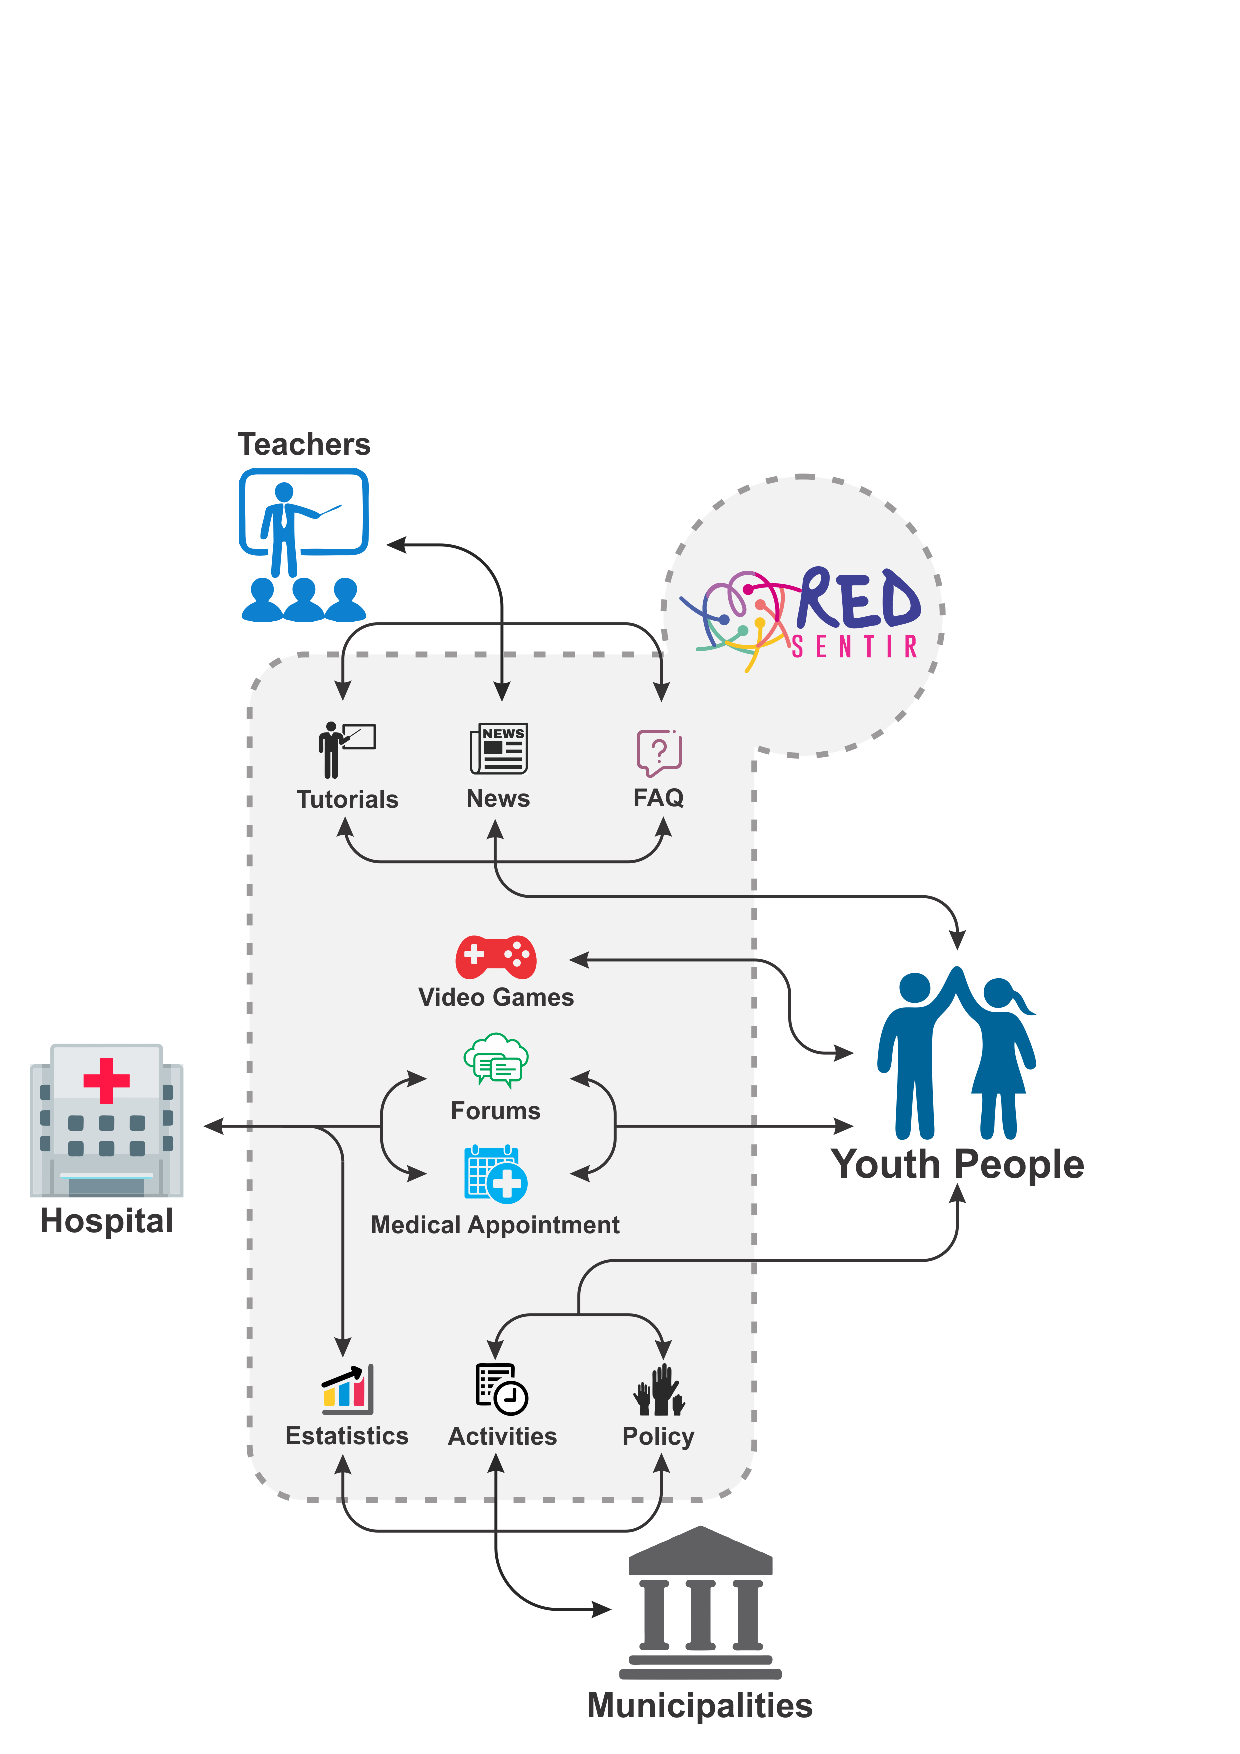
\includegraphics[width=0.3\textwidth]{Digital_Platform.png}
\caption{Structure of the Red sentir.}
\label{fig:estructura}
\end{figure}
 
For the creation of the Red Sentir digital platform it was necessary to carry out a series of steps that would allow to go structuring and at the same time to give the required functionality to the platform; in the following descriptions it is provides in greater detail the steps taken:

\textbf{$(i)$ Development of the base structure of the platform of the Red Sentir:} Based on the design pattern MVC is created the base structure of the documents of the platform, on this basis a template folder is defined (created), that contains another folder named ``sitio'' where they are located separate way sub-folders that contain templates or models for each of the modules that are part of the project. Within the templates folder is included, in the root of the directory, the base.html document that constitutes the support of the presentation of the platform. It is defined in addition the static directory where all the documents are located of the platform, i.e., the images, audiovisual contents, style files .css, the code to be executed on the client's side i.e. the documents.js javascript and the constructions of the available games inside the platform. A directory was also created (or application) for each module with the respective controllers and models, as well as a directory (or project) called a ``red sentir'' to contain the configuration documents and system urls. A security module that contains the controllers and user models and user profile in addition to the methods for creating and editing users.

\textbf{$(ii)$ Settings.py:} The document setting.py correspond to all the configuration of the “Red Sentir” platform, in it the database configured in Postgresql is related, it is configured the root route, the static route, the communication mail it is configured, the different applications are added and the login is redirected directly to the timeline. The document is on the route: redsentir/server.py.

\textbf{$(iii)$ Creation of the relational tables with the database through Postgresql:} The platform of the “red sentir” uses relational databases where each of the relationships must be created through the Structured Query Language (SQL), in order to go linking the different users and contents of the platform.

\textbf{$(iv)$ creation of registration form:} It is created in html language and a ccs registration form through which the users that enter the platform can fill all the corresponding information for the creation of their profile, the basic data to carry out this, are. $(i)$ the username, $(ii)$ the date of birth, $(iii)$ the password, $(iv)$ the email, $(v)$ the phone number, $(vi)$ the sex, and $(vii)$ the avatar choice. All these data will identify you within the system. The birth date is of special importance, because through this information a separation and consultation process it is carry out in this database for the differentiated visualization within the digital platform “Red sentir”~\ref{fig:vista_plataforma}.

\textbf{$(v)$ Creation of authentication form:} It is created in html language and a ccs an authentication form through which the users who enter the platform identify themselves with their corresponding user and password.

\textbf{$(vi)$ Creation of a user profile model:} since the platform design follows the MVC, it is necessary to implement the user profile model with the corresponding fields where the data type and the default values are also defined.

\textbf{$(vii)$ Administrator of Django:} The administrator allows controlling the other modules of the system such as the security module, which is where the users of the platform are registered, as well as the groups of permits that are registered, assign these users. The administrative module is developed at the same time as the other modules, because it facilitates the creation of test entities through the methods that allow creating, removing, editing and listening the instances of objects in each case, it has an authentication and authorization menu for the creation of users and groups. Within the module it is also possible to administer what is added in several of the existing modules, thus allowing to control in a simple way the content that is published. The modules that can be modified from the administrator, either to upload, delete or edit, are: $(i)$ frequent questions with their respective answers $(ii)$ training through the ability to add and edit the meetings, $(iii)$ forums, $(iv)$ regional bureau plans, $(v)$ security, $(vi)$ users and groups, and $(vii)$ young friendly health services. 
%In the figure~\ref{fig:admin} shows a brief view of the administrator module of the “Red sentir”.

It is through the configuration of these steps that the visible modules within the platform and their functionality can be built.

\subsection{Platform modules}

\textbf{$(i)$ Novelty:} A new module was created that works as a timeline where young people can participate through multiple tools: text, audio, image or video. One of the added values of this module is that it is only available to young people, so the interaction occurs directly between them, allows them and gives them greater confidence to express their opinions and express themselves. 
%Figure~\ref{fig:novedades} shows the view of the module.

\textbf{$(ii)$ Young friendly health services::} A module of young friendly health services was created, this module consists of a tool that enables and approaches teenagers with municipal health centers and professional aids in matters of promotion and prevention, this module is considered a mechanism of technological transfer to hospitals, since it allows to improve the access to health services and the opportunity for care, as well as the possibility for young people to perform supervision and control of these services through the qualification they give to the services they access. 
%Figure~\ref{fig:SA} shows the view of the module.

\textbf{$(iii)$ Frequently questions:} The frequently questions module was created so that teens can easily find the answers to common questions, many of them are identified from the line of support of the formation processes that have allowed, the construction of the content of this module, hence the importance as it provides an answer to contextual needs, these questions are prioritized according to the number of times they are consulted by the young people in different spaces. 
%Figure~\ref{fig:FAQ} shows the view of the module.

\textbf{$(iv)$ Forums:} The forum module was created so that the users of the platform can interact and ask directly experts from the health or psychology area who can solve the questions they do not find within the module or frequently asked questions (otherwise the young people would have limited access to this type of information). To make the young people feel confident when they participate in the forums, the anonymous button is implemented, which allows participating in the forums and the user name does not appear in the comments of the forum, figure~\ref{fig:foros} shows the view of the forum module.

\textbf{$(v)$ Videogames:} Taking into account the different digital strategies oriented to education, as it was stated in~\ref{videojuego}, within the ``Red sentir'' the creation of a videogame that would link the subject of sexuality was planned, and that at the same time it allows them to learn by having fun. Two videogames were programmed to deal with and address these issues from two different approaches, the first one is based on the type of game ``endless runner'', the game is called ``Preventor'' and the idea is to prevent the sperm that are appearing from touching the ovum which is manipulated by the player, the game ends when the measure of energy reaches $0$. The second is based on ``castle defense'', and is called ``Dawn of Zoides'', in which the dynamics of the game it consists of preventing the sperm from reaching the castle. The Figure~\ref{fig:juegos} shows ones of the two games available within the ``Red sentir'' project.

\textbf{$(vi)$ Formation:} It was created a formation module in which is related the material and the methodology used in the courses, so teachers can reply the strategies to aboard the sexuality topic with the students since they have at their disposition the guides made by the training component. In addition, the module shows the reviews of the meetings held in which intergenerational dialogues were given, the formation module can be seen in figure~\ref{fig:formacion}.

\textbf{$(vii)$ Regional Bureau:} This regional bureau module makes a relationship of all the commitments that were reached with the participant institution in the local and regional bureau in the municipalities that are part of the ``red sentir''. The importance of the regional bureau within the ``red sentir'' lies basically in the fact that a project like this makes sense as long as various actors involved get to know and support each other from the possibilities of each one, recognizing this space of the platform and making participants of the same, either through the implementation of strategies, an event dissemination space or a complement to the local strategies themselves.

\textbf{$(viii)$ baseline:} Within the baseline module the results of the diagnosis are displayed, socio-demographic aspects, social activities, personal relationships, sexual health, life plan, subgroup analysis and adolescent pregnancy within the regions that understand the project. The way in which the module is presented is shown in figure~\ref{fig:lineabase}.

Within the results obtained in the development of the project, and which can be viewed in the digital platform are: $(i)$ a platform made to measure in operation, $(ii)$ two video games on the platform, $(iii)$ pedagogical materials with virtual access, $(iv)$ $30$ virtual forums for the participation of adolescents, $(v)$ information on the project on the platform, $(vi)$ manifestation of the commitments of the municipal mayors, $(vii)$ linkage of the health service providers of the municipalities, and $(viii)$ constant accompaniment and solution of concerns to young people through the digital platform.

The digital platform of the ``Red Sentir” In the first six months of operation, it has achieved a total of 2511 users ($52\%$ men, $44\%$ women and $4\%$ did not select).

To observe the web application developed by the digital component of the ``Red Sentir'', it is necessary to enter the browser~\url{www.redsentir.org}, there you can see the different results exposed in the present article.

\begin{figure}[tbp]
\centering
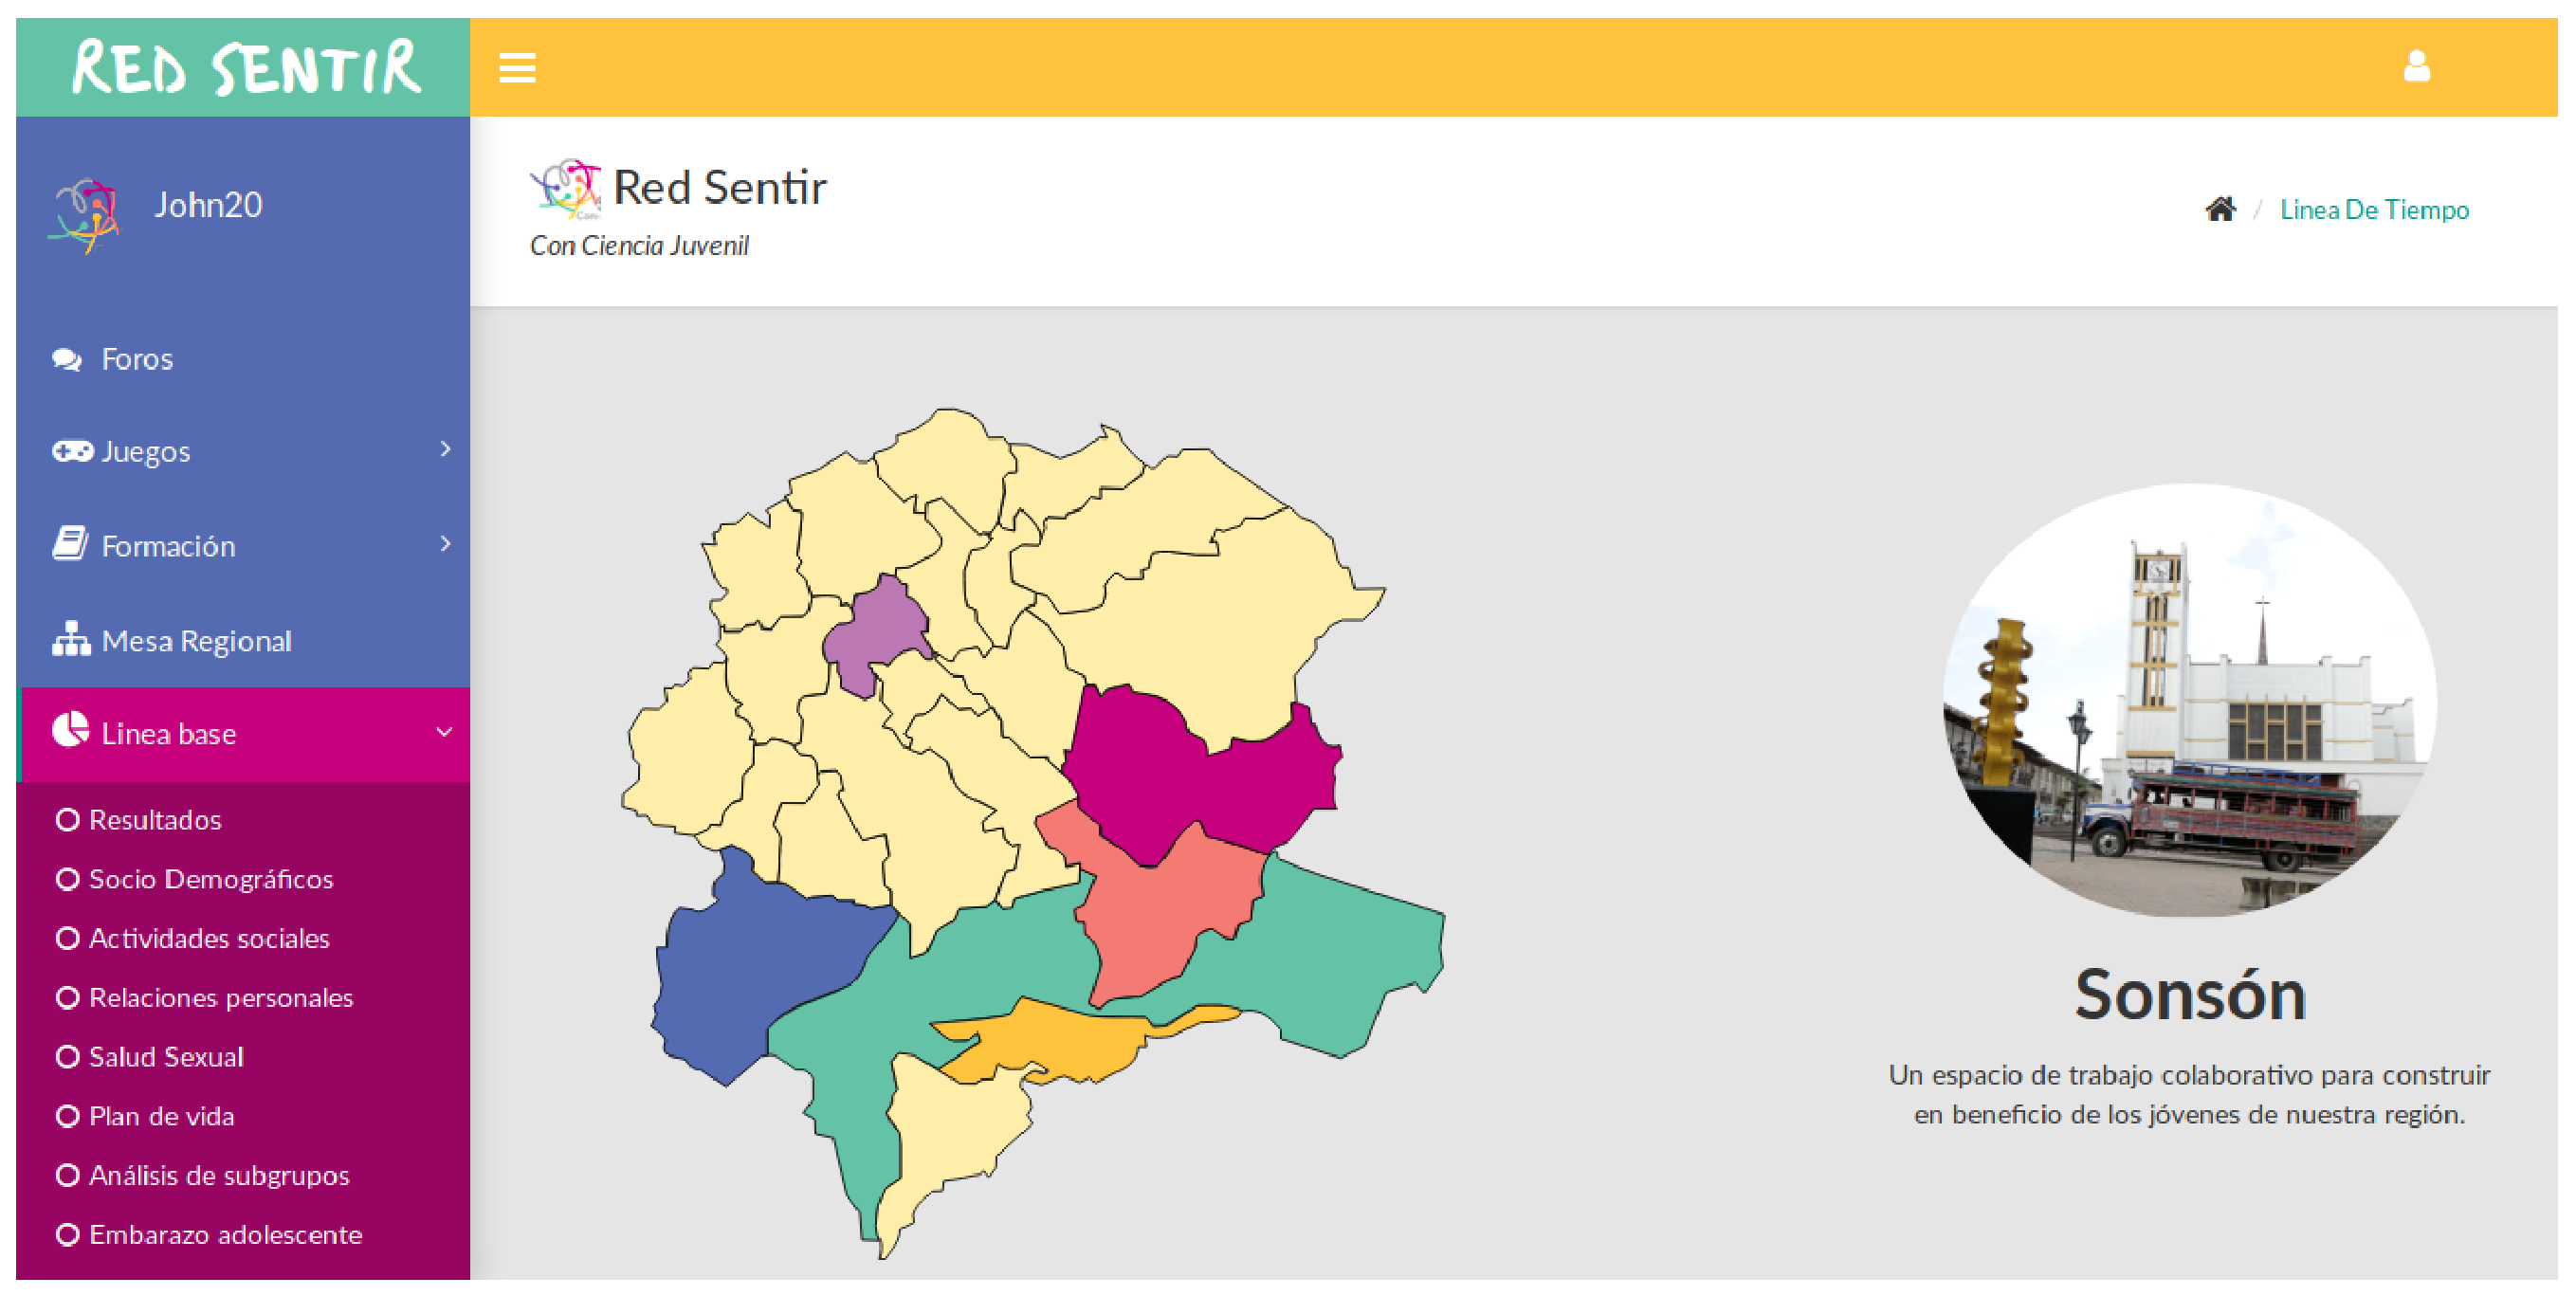
\includegraphics[width=0.48\textwidth]{mayor.eps}
\caption{The view of the digital platform changes according to the age of the user.}
\label{fig:vista_plataforma}
\end{figure}

%\begin{figure}[tbp]
%\centering
%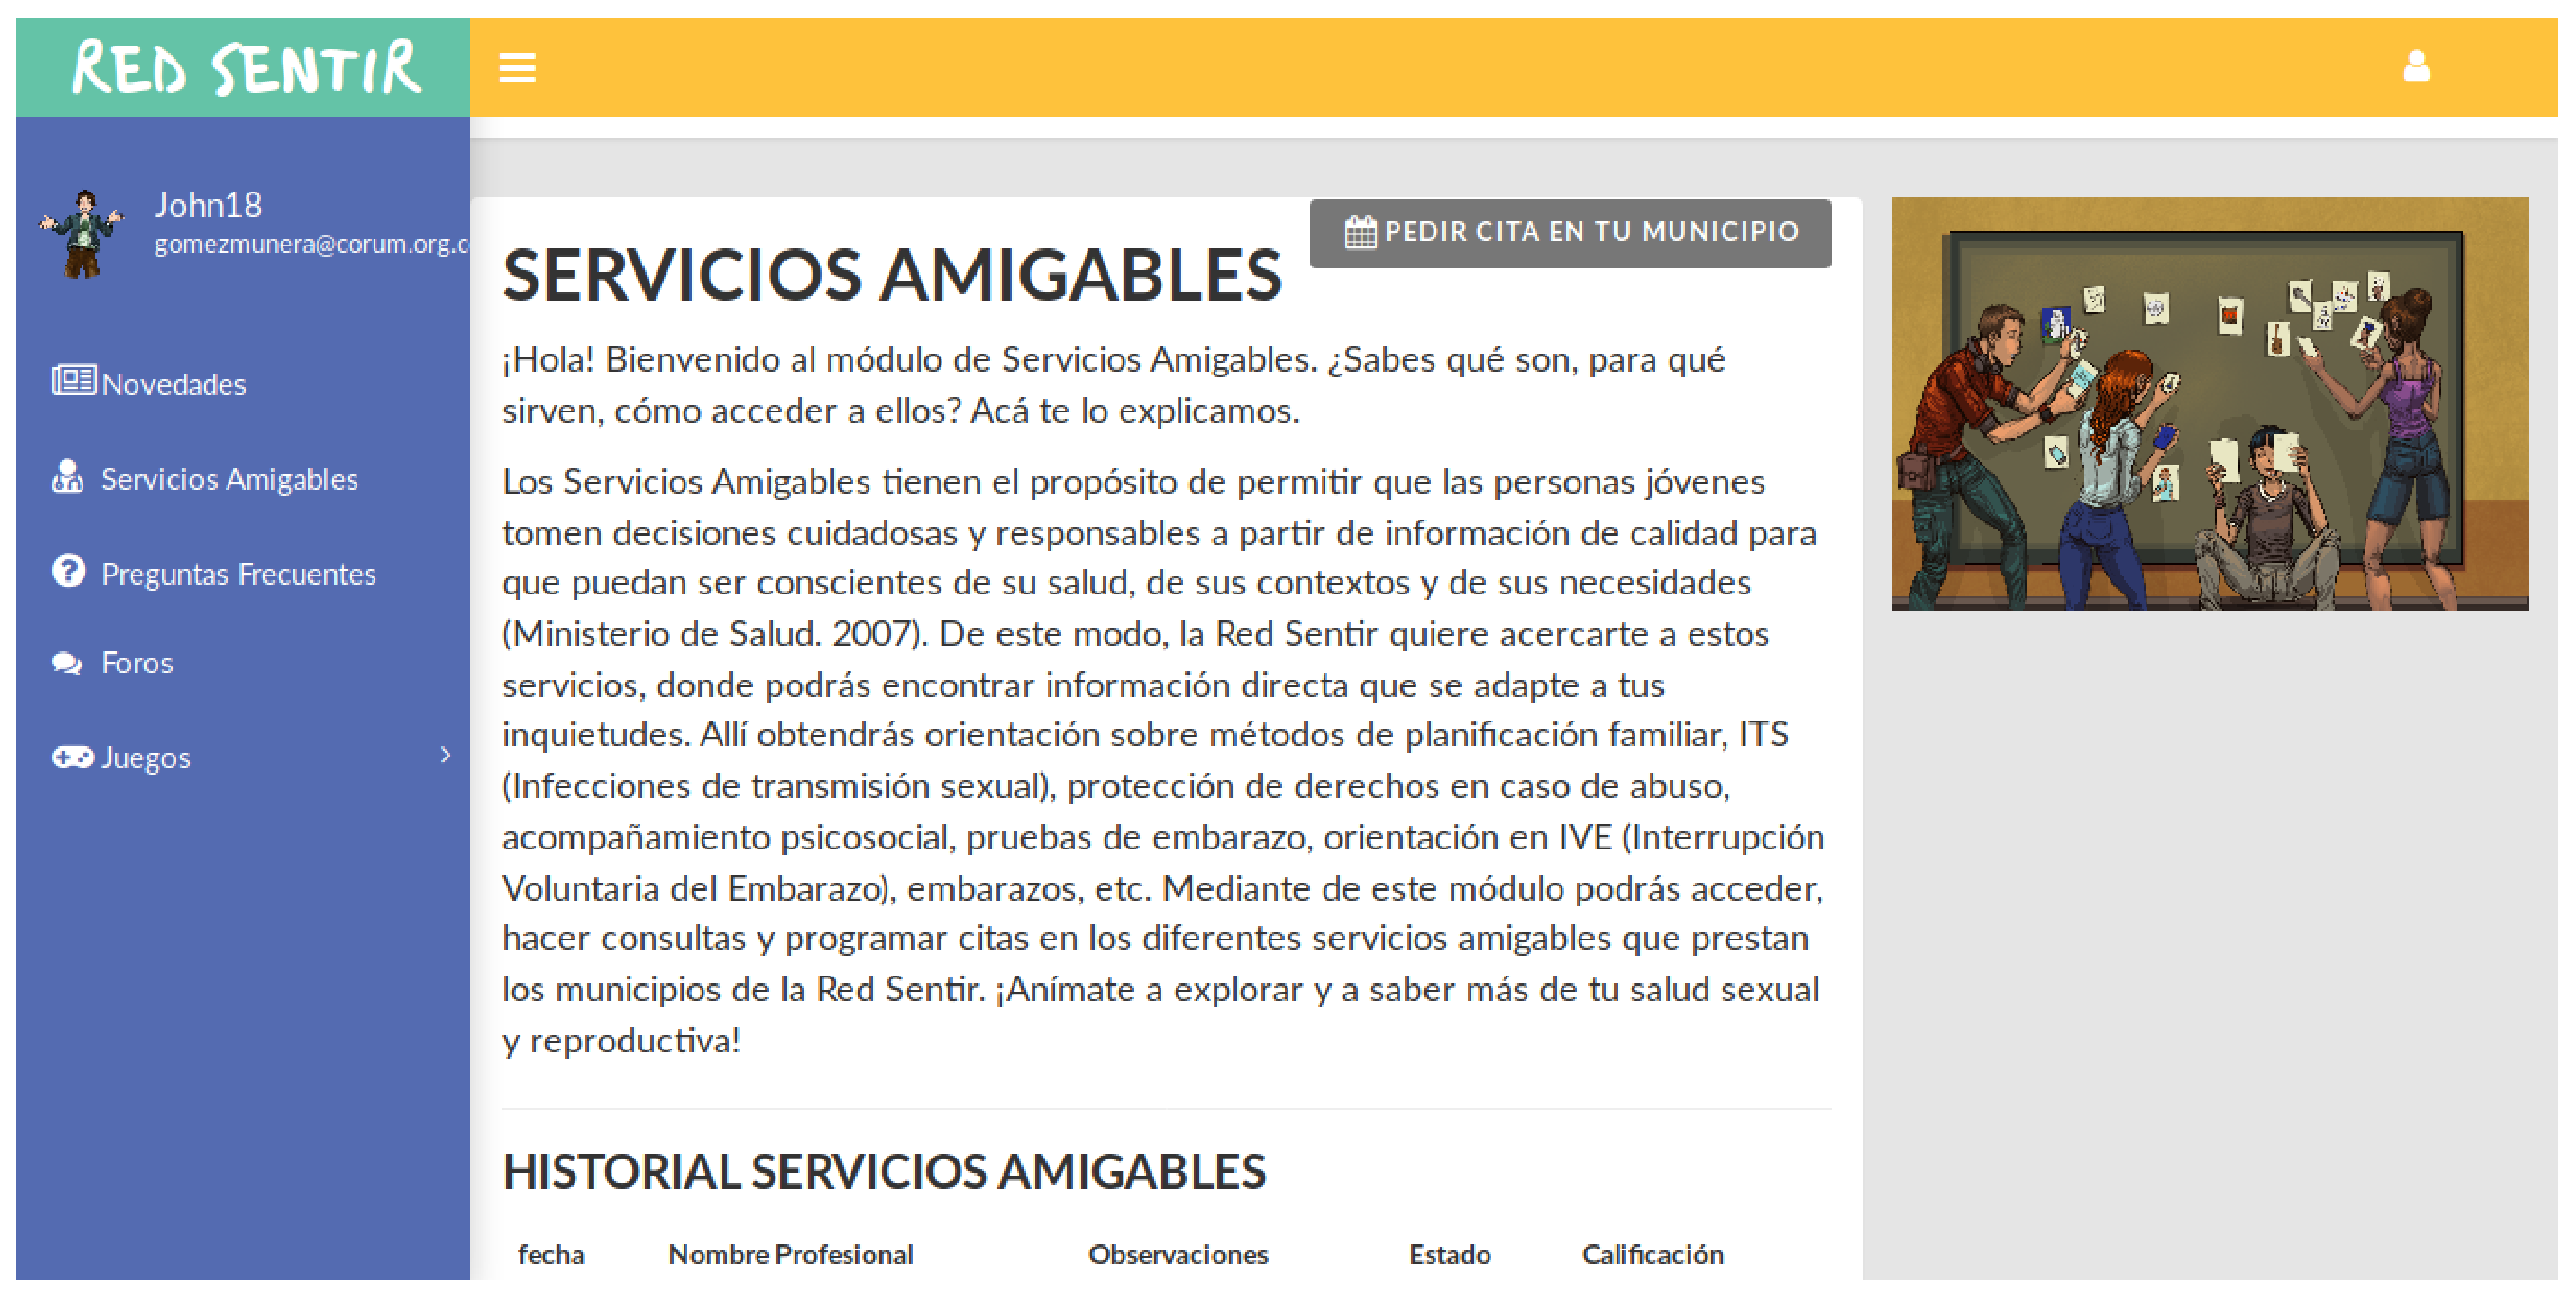
\includegraphics[width=0.48\textwidth]{SA.eps}
%\caption{Young Friendly Health Services Module.}
%\label{fig:SA}
%\end{figure}

%\begin{figure}[tbp]
%\centering
%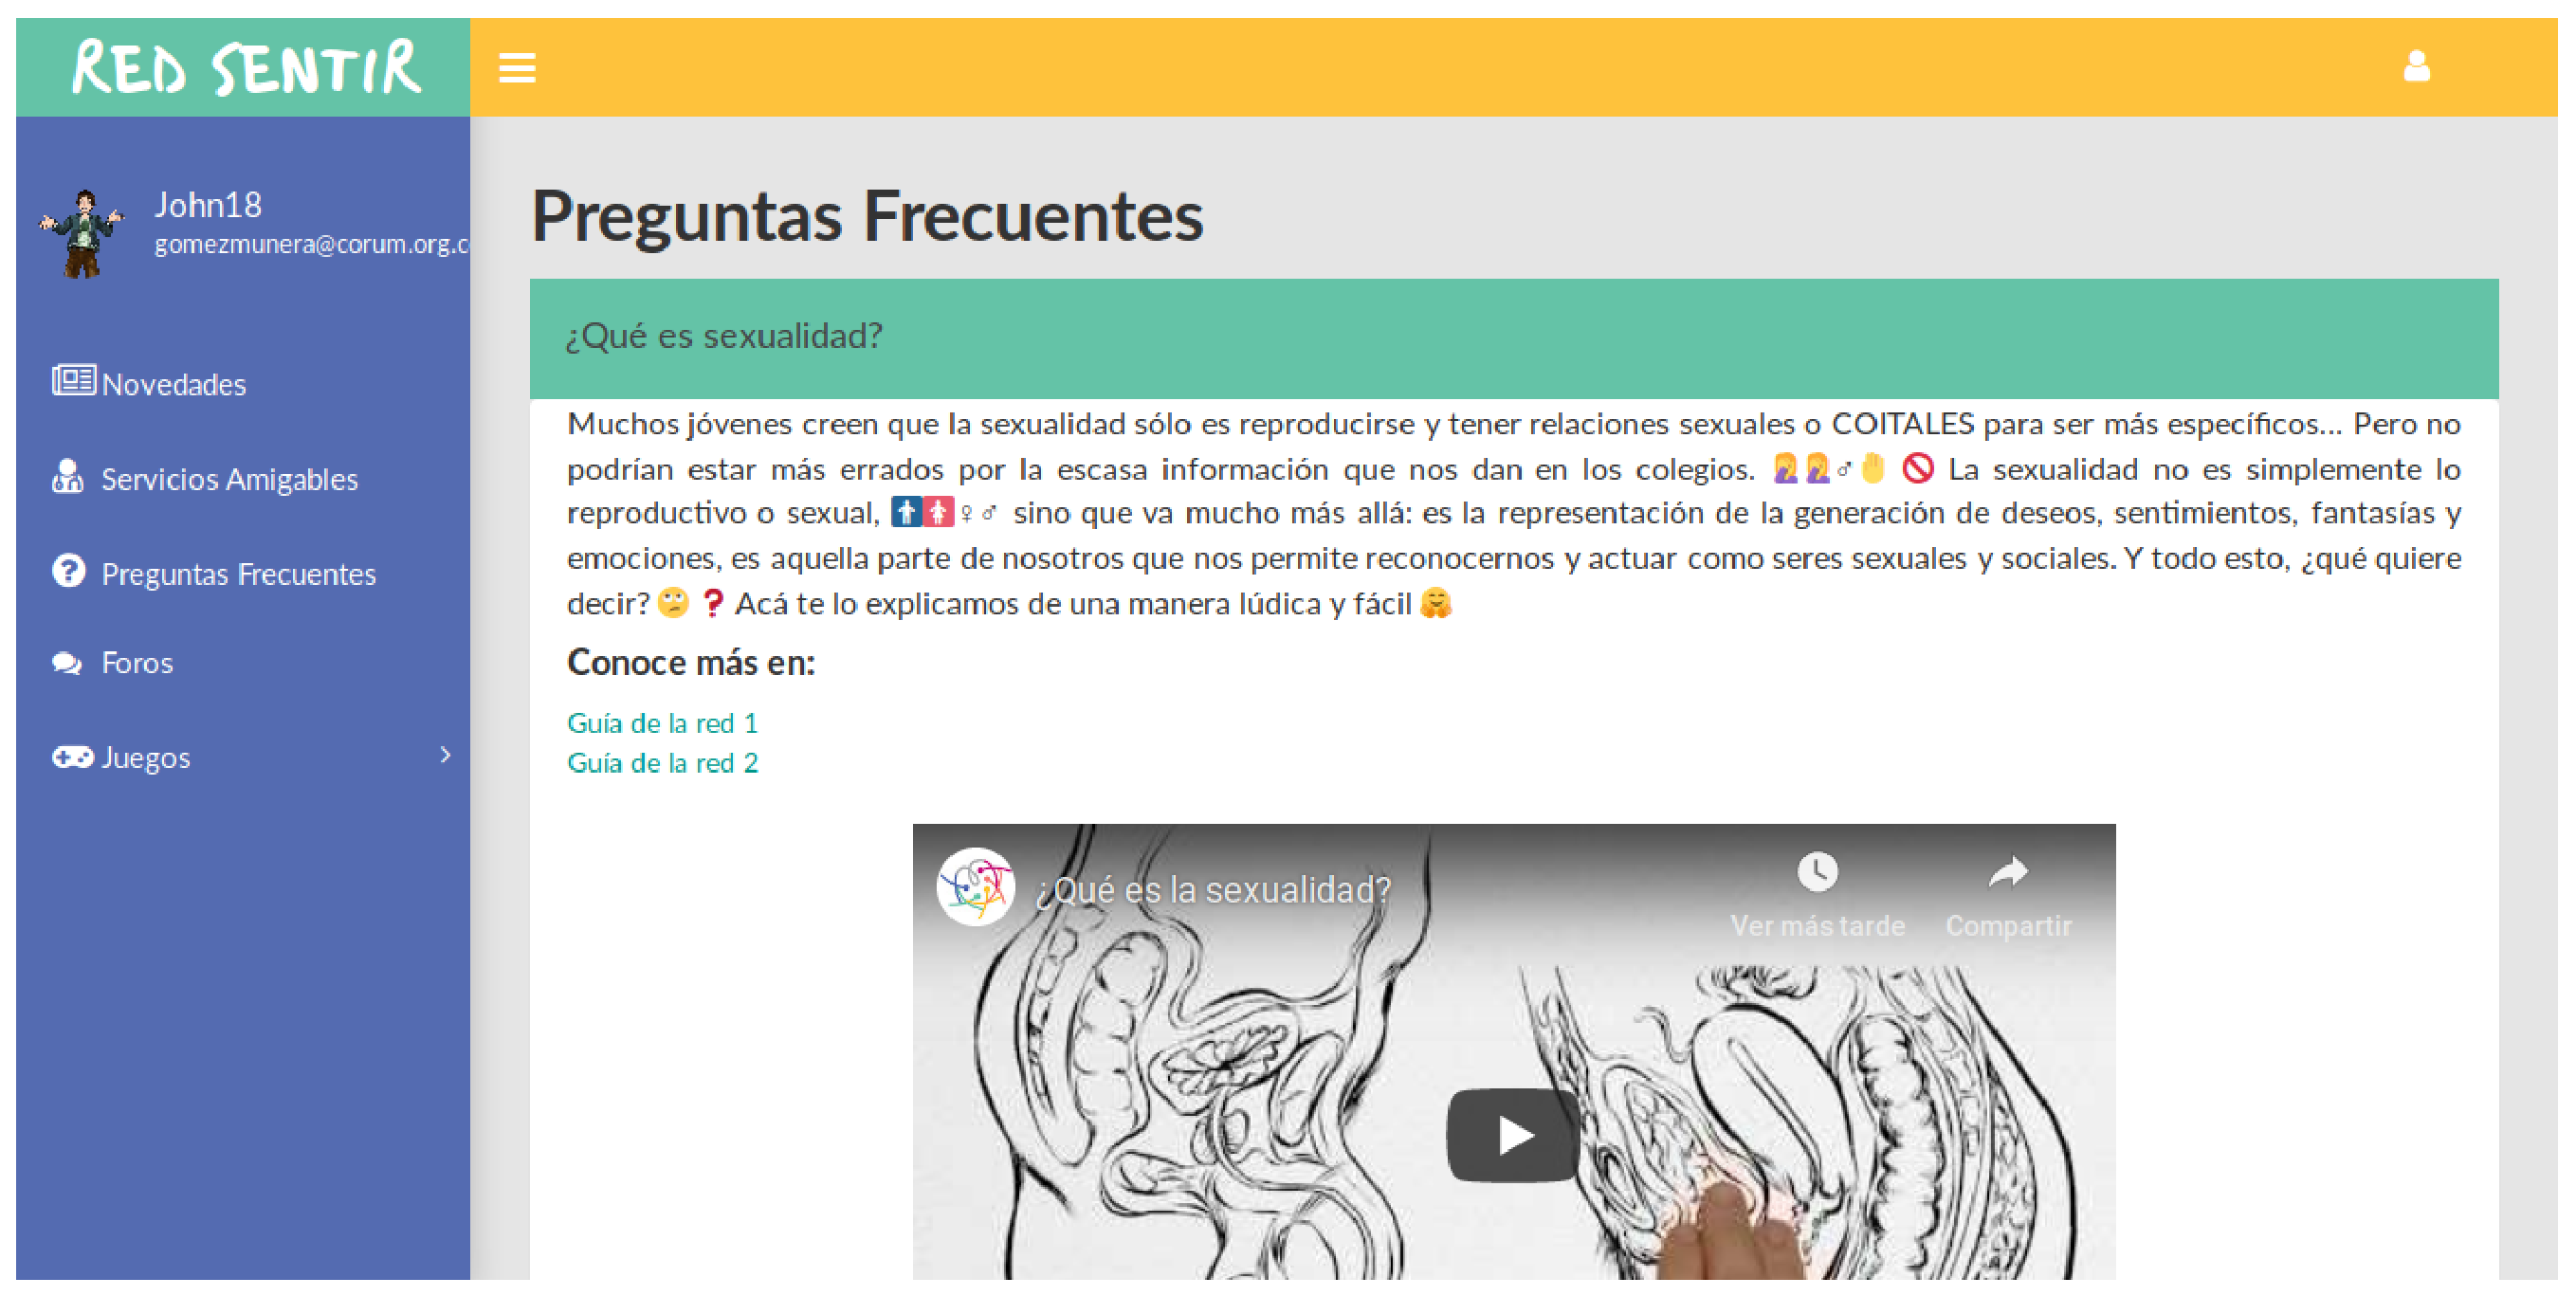
\includegraphics[width=0.48\textwidth]{FAQ.eps}
%\caption{Frequently are asked Questions Module.}
%\label{fig:FAQ}
%\end{figure}

\begin{figure}[tbp]
\centering
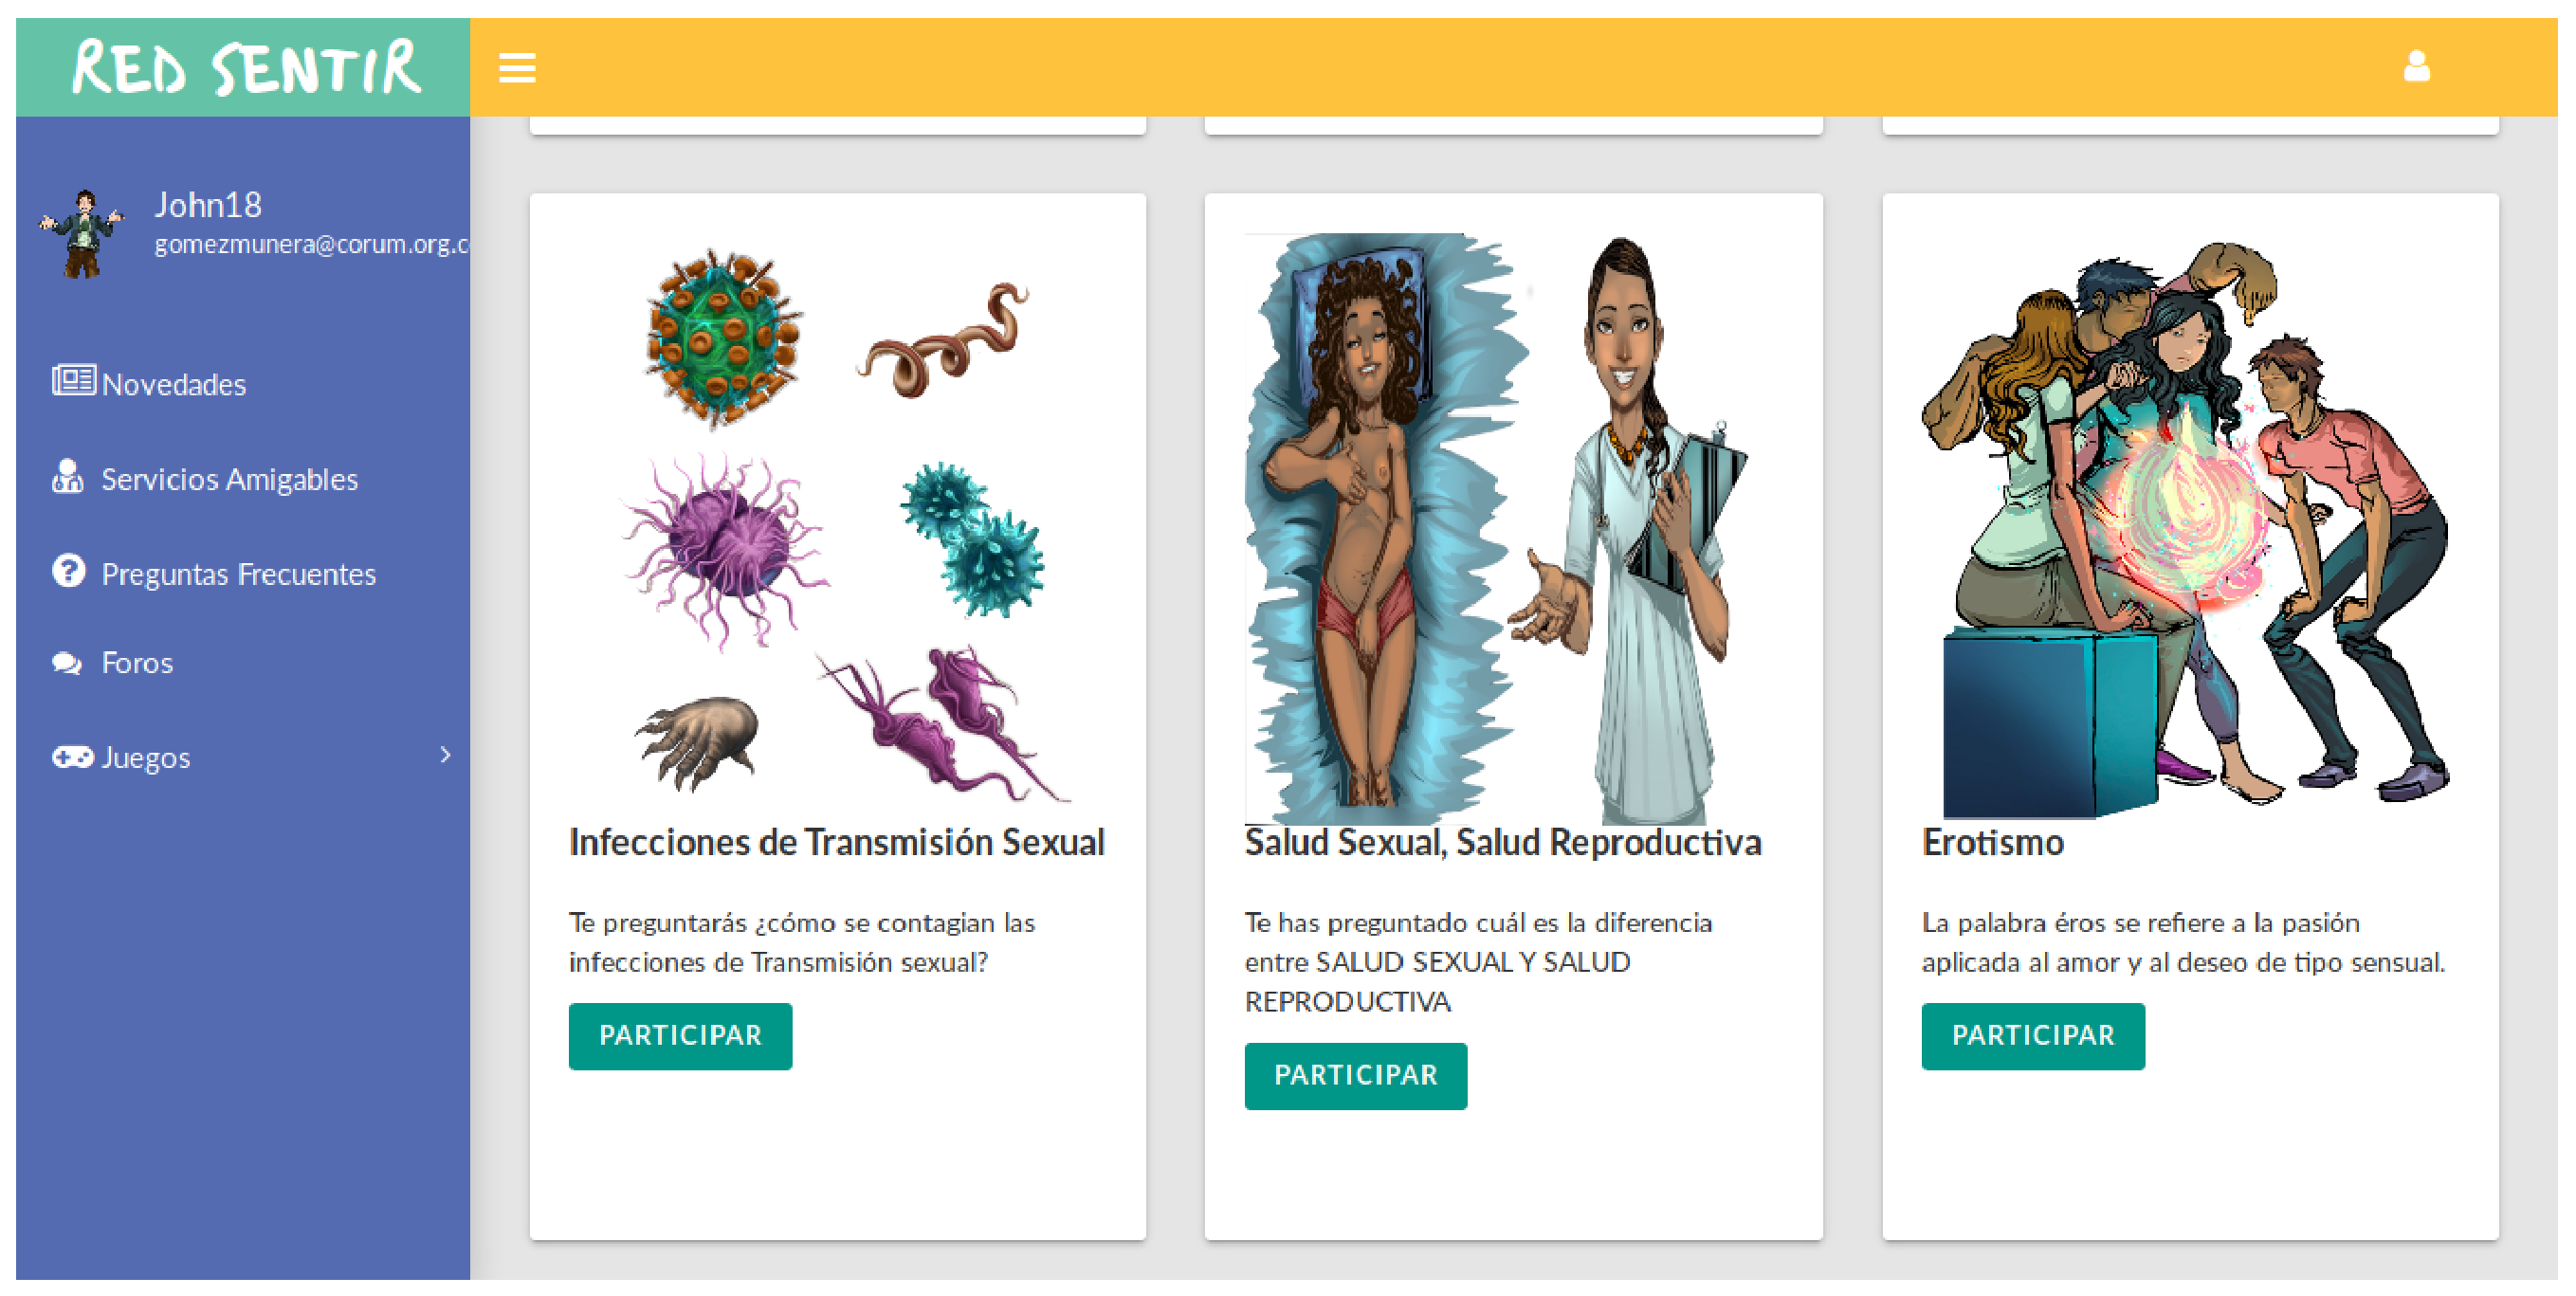
\includegraphics[width=0.48\textwidth]{foros.eps}
\caption{Forum module of the ``Red Sentir''.}
\label{fig:foros}
\end{figure}

\begin{figure}[tbp]
\centering
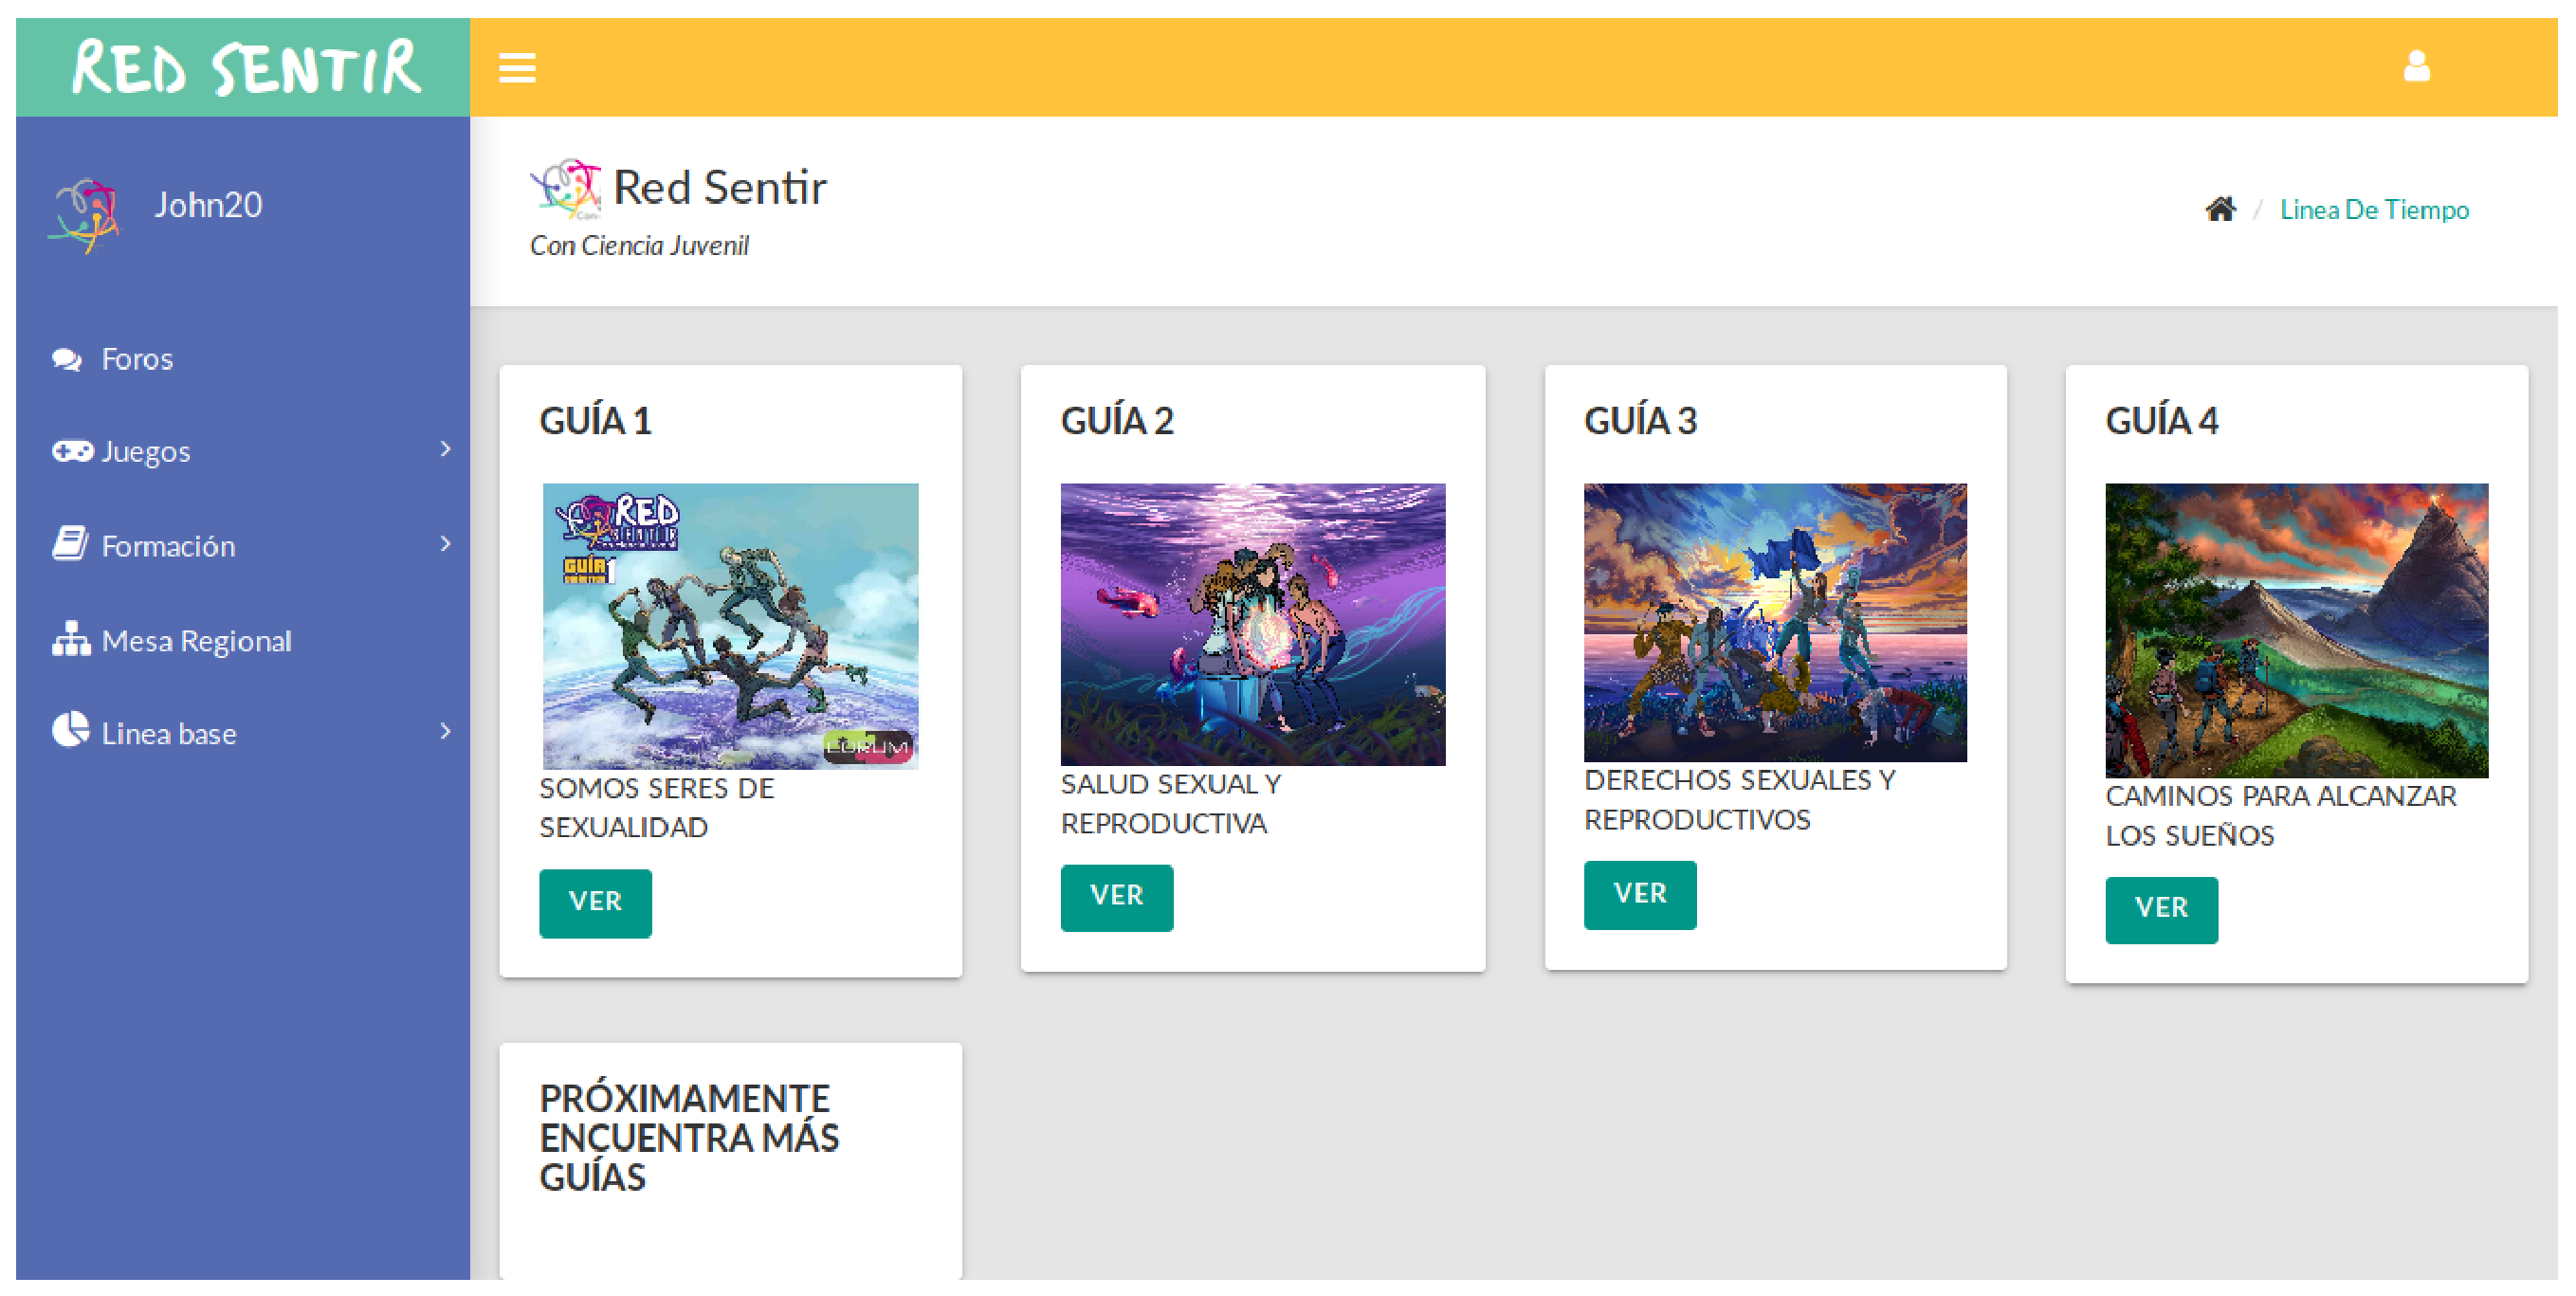
\includegraphics[width=0.48\textwidth]{guias.eps}
\caption{Formation module available on the platform.}
\label{fig:formacion}
\end{figure}

\begin{figure}[t]
\centering
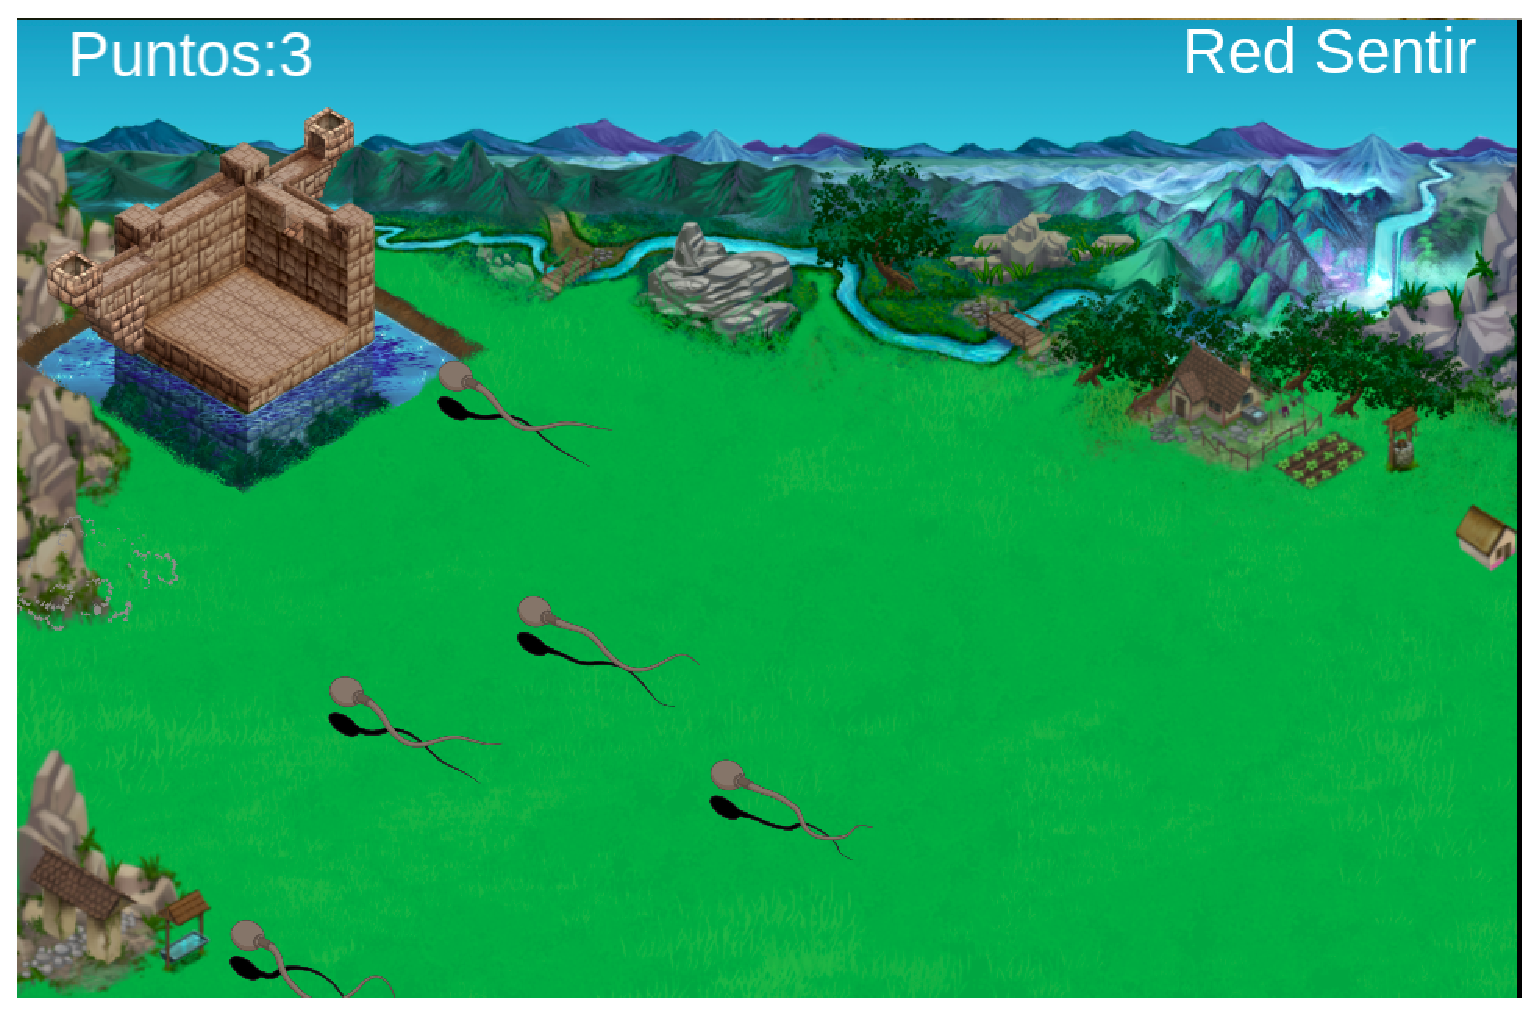
\includegraphics[width=0.4\textwidth]{juego2.eps}
\caption{Videogame available on the digital platform of the ``Red Sentir''.}
\label{fig:juegos}
\end{figure}

\begin{figure}[t]
\centering
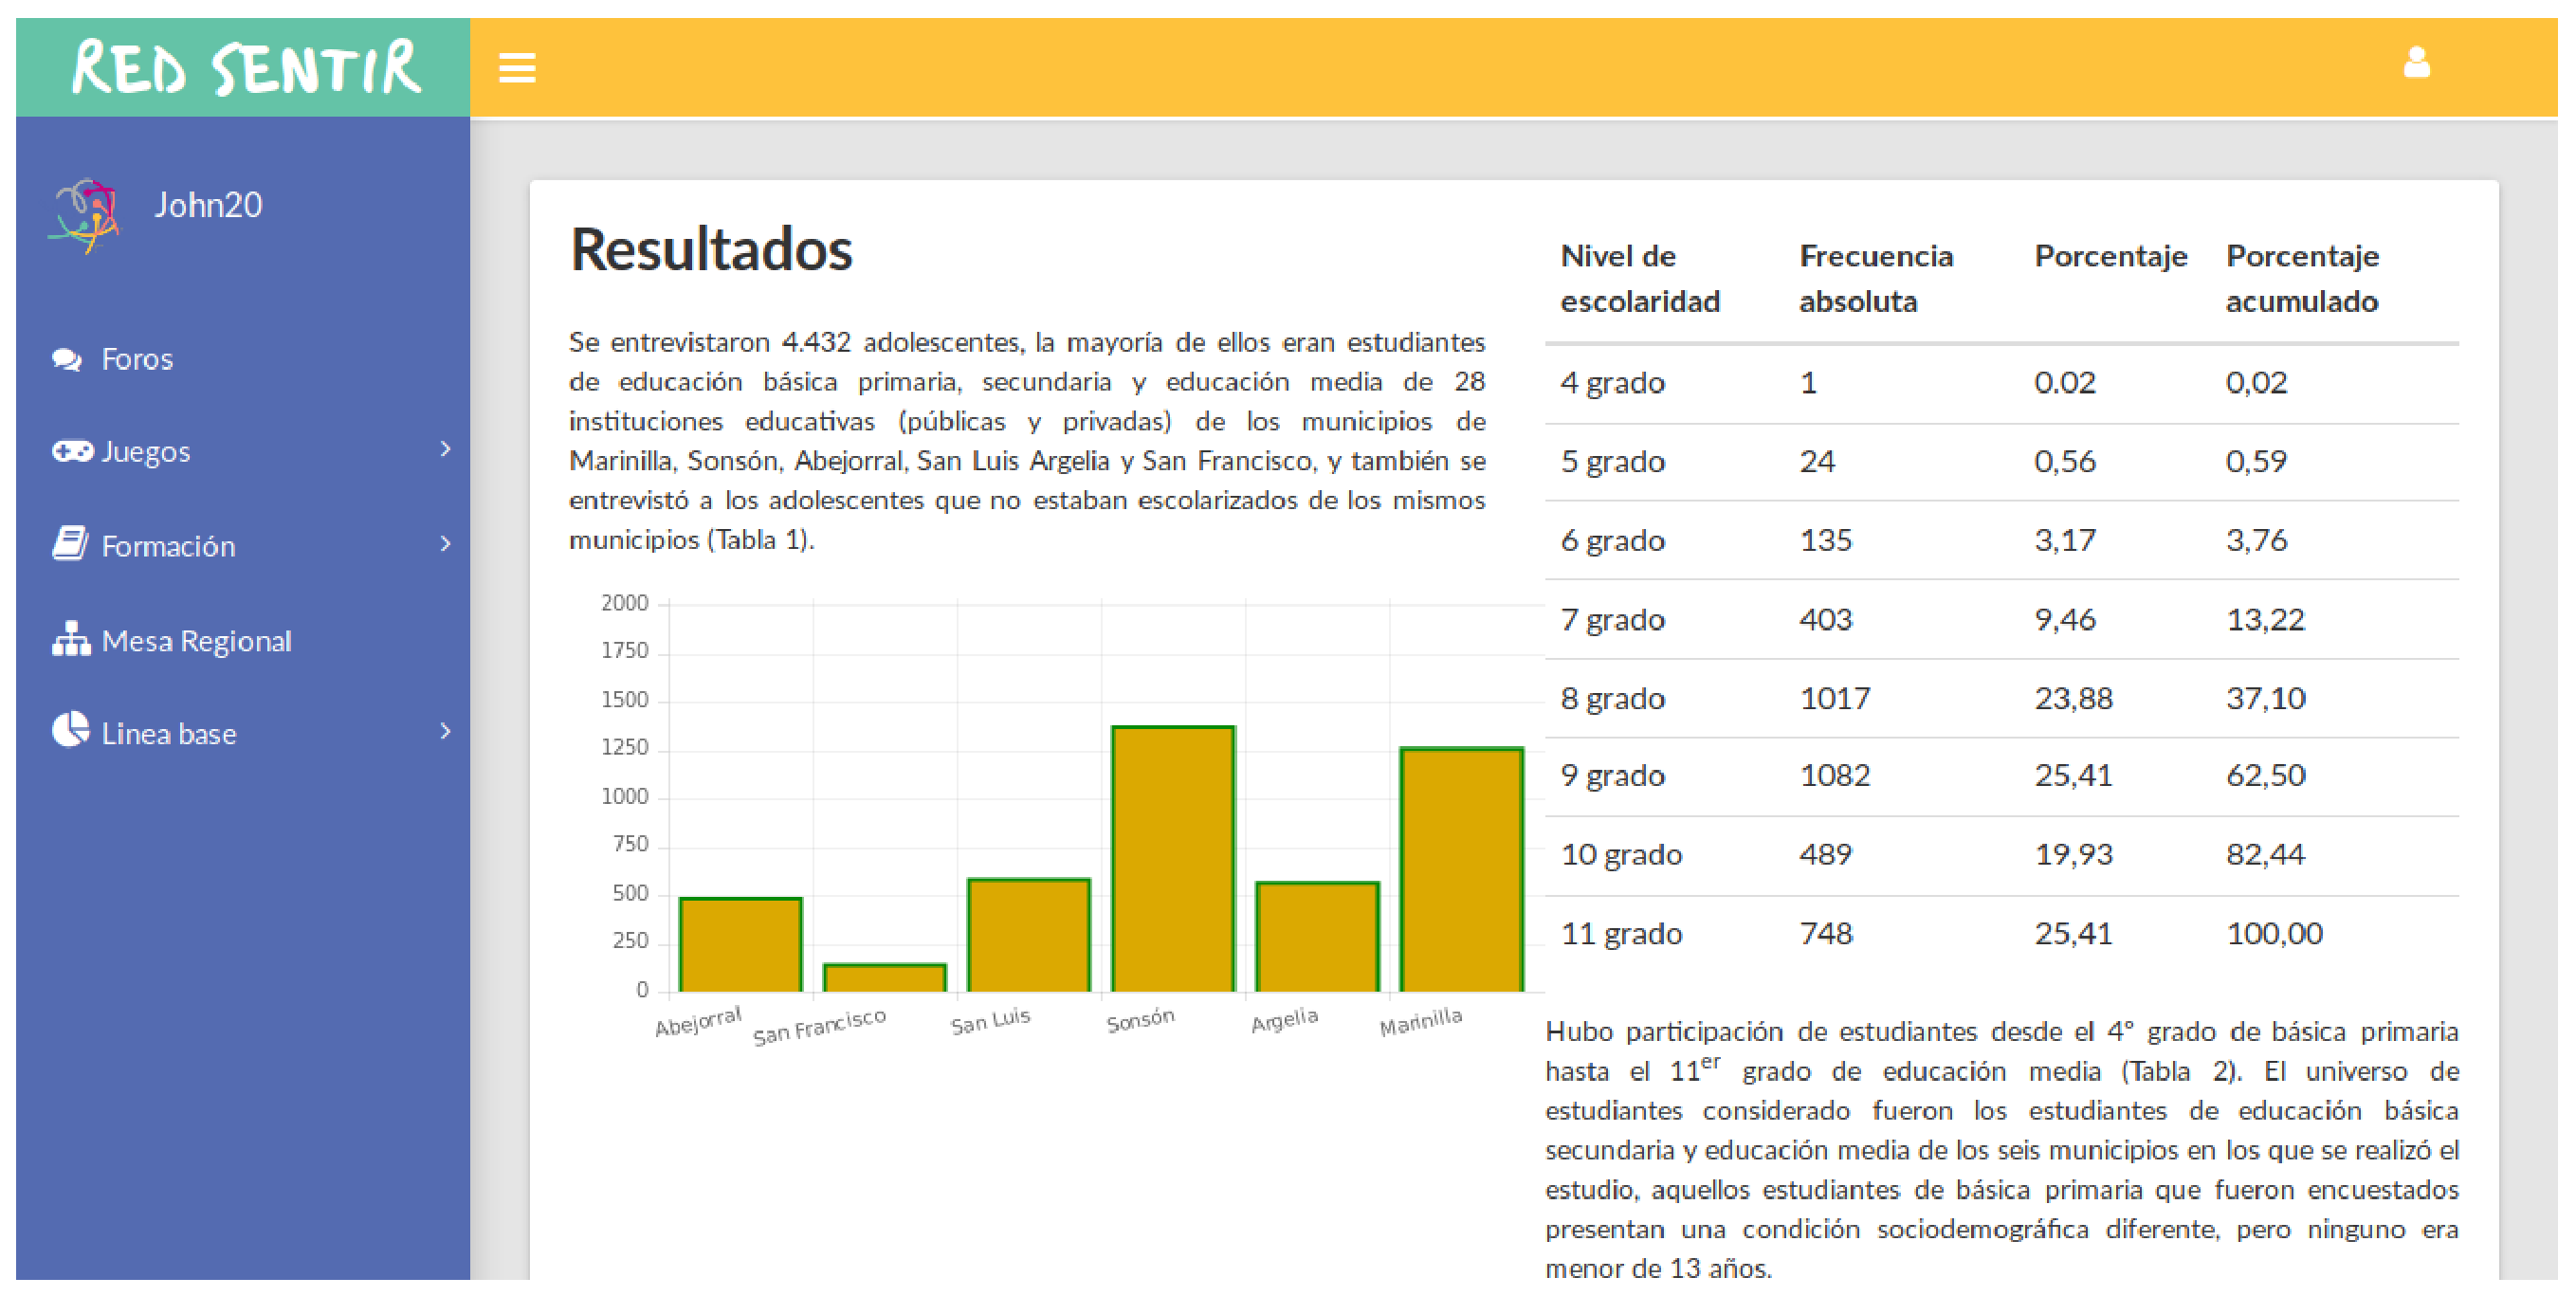
\includegraphics[width=0.48\textwidth]{resultados.eps}
\caption{Module of the baseline of the project.}
\label{fig:lineabase}
\end{figure}

\section{CONCLUSIONS AND PERSPECTIVES}\label{sec:conclusiones}
The Red Sentir has become a novel strategy for the approach of the adolescent pregnancy phenomenon. Phenomenon resulting from various problems and characterised as a phenomenon of high complexity (UNESCO). Responding to this complexity requires the articulation of actions of different institutions in such a way that they can be create favorable social impacts, it is like the platform Digitalof the Red Sentir responds to these needs and created digital tools to facilitate complex interactions between governments, schools, youth, teachers, institutions of health and the team of the Red Sentir.

The Red Sentir meets the search for national governments to generate greater inclusion the risk factors in which are immersed in many of the people, which end in many cases consequences that may truncate the life plan of the young people perpetuating the cycles of poverty in the communities. In the same way, it is not only the economic situation that is the one influences the educational processes of adolescents, but also the demographic, social, cultural factors and one what is more important is access to ICT, since of it that you can improve the living conditions of people through digital strategies stories like digital platform of the Red Sentir.

With the research carried out by Red Sentir about the risk factors associated with the pregnancy phenomenon adolescent is an intervention strategy in doing emphasis on the planes of life, human rights, the recognition of the territory, the care of the body, the use of contraceptive methods and strengthening of dreams.

The virtual platform is complemented with the process carried out done by the training component as a strategy to link, improve and achieve a different scope to achievement with adolescents who directly participate in the courses, in addition the linking of the forums allows provide information idoneous in contexts where the expert does not it can come to another form.

%The implementation of the platform in social areas worked allowed them to generate a greater appropriation in the thematic issues addressed through the tools and the use of ICT, in particular from the digital platform of Red Sentir, which has also allowed the documentation process in and registration so that it can be replicated in different contexts not only national but also international.

From the technical point of view, the use of different frameworks allowed the programming of a virtual platform whose objective is to create trust in the youngest ones, by functioning as a social network oriented directly to work, talk and train on sexuality issues, so that young people can get information that helps them to experience, discover and live sexuality in a responsible way. With the development of the digital platform, it was possible to incorporate and mix technologies together with the respective languages used that led consistently and in good terms to a final result reflecting the strengths and the interdisciplinary character of the Red Sentir team.

Both the products and the results obtained by the project, they give a positive and satisfactory analysis in all the aspects and from the different components. That shows in itself, the establishment of a base to continue intervening in communities where this risk factor is high, leaving in itself a job that can be extended, complemented and replicated for the other communities in which it is considered pertinent to implement the strategy. Within the functionalities that the digital platform can have, the they can be extended and incorporate new tools, since this is a task of continuous growth that should adapt to new technologies, being an iterative and incremental process, although that is precisely that which can be seen as an opportunity, since within the digital, the need to introduce new improvements and new content that complement what has already been implemented is what allows generate a trust and a return to the platform, between identified functionalities to continue working within the platform:

\begin{itemize}
\item Create continually content for young people, parents and institutional actors.
\item Turn it into a massive tool, that is implemented in educational institutions within a national ambit, serving as a support in the teaching of sexuality.
\item Link educators to generate collaborative work through the platform.
\item Improve and update existing video games within of the platform, increase the difficulty of the video games as they become is progressing and getting points. Said difficulty it can be reflected in higher speed, apparition of new characters, use of different tools, movements, including new animations, inclusions of educational information or new graphs.
\item Have a commercial strategy for purchasing elements that help self-care and prevention
of pregnancy (Contraceptives), with the aim of being offered through the platform and generate sustainability financial for it.
%\item Have a record of the scores obtained in the video games within the database, which would allow having a better statistic of the users and level of play, for perform subsequent treatments.
\end{itemize}

\bibliographystyle{IEEEtran}
\bibliography{biblio_digital}
\end{document}
